\section{Ziel}
\label{sec:Ziel}

Ziel des Versuches ist die Bestimmung der Suszeptibilitäten
verschiedener paramagnetischer Oxide seltener Erd-Elemente.\\
Dazu wird eine Brückenschaltung verwendet.\\ 

%\cite{sample}

\section{Theorie}
\label{sec:Theorie}

\subsection{Magnetische Suszeptibilität}

Die magnetische Suszeptibilität $\chi$ gibt Auskunft darüber, wie sehr sich 
die Magnetisierung $\vec{M}$ des Stoffes in einem äußeren Magnetfeld ändert.\\
$\chi$ ist dimensionslos und hängt von verschiedenen Parametern, wie der magnetischen Feldstärke
$\vec{H} = \frac{1}{\mu_0} \vec{B}$ und der Temperatur $T$ ab. Die Magnetisierung lässt sich durch
\begin{equation*}
    \vec{M} = \mu_0 \chi \vec{H}
\end{equation*}
berechnen.\\
Bei Raumtemperatur und in einem kleinen Magnetfeld $\vec{B} < 1 \mathrm{T}$ sind die Suszeptibilitäten
näherungsweise konstant. \\
Stoffe, deren Suszeptibilität unter Null liegt, sind diamagnetisch. Unter Einwirkung eines äußeren Magnetfeldes
magnetisiert sich ihr intrinsisches entgegengesetzt zum äußeren Feld, sodass 
das Magnetfeld im Inneren des Volumens schwächer ist als außen. \\
Wenn die Suszeptibilität eines Stoffes über Null liegt, ist er paramagnetisch. 
Das innere Magnetfeld ist bei einem extern anliegenden Magnetfeld stärker als das externe, anregende Magnetfeld.\\



\subsection{Suszeptibilität paramagnetischer Stoffe}

Paramagnetische Stoffe haben einen nicht verschwindenen Drehimpuls.\\
Der Gesamtdrehimpuls $\vec{J}$ setzt sich aus dem Gesamtspin $\vec{S}$ und der Summe $\vec{L}$ der Bahndrehimpulse sowie dem Kerndrehimpuls zusammen. Der Kerndrehimpuls kann in diesem Versuch für den Paramagnetismus vernachlässigt werden.\\
Ist die Elektronenschale mehr als halbvoll besetzt, gilt $\vec{J} = \vec{L} - \vec{S}$, sonst $\vec{J} = \vec{L} + \vec{S}$.\\

Mit den Beträgen der magnetischen Momente 
\begin{equation*}
    |\vec{\mu_L}| = -\mu_B \sqrt{L(L+1)}\ \textrm{und}
\end{equation*}
\begin{equation*}
    |\vec{\mu_S}| = - g_s \cdot \mu_B \sqrt{S(S+1)}
\end{equation*}
lässt sich die Beziehung 
\begin{equation*}
    |\vec{\mu_J}| = |\vec{\mu_S}| \cdot cos(\alpha) + |\vec{\mu_L}| \cdot cos(\beta)
\end{equation*}
herleiten und zu 
\begin{equation*}
    |\vec{\mu_J}| \approx \mu_B \cdot g_J \sqrt{J(J+1)}
\end{equation*}
approximieren.\\
Hier sind $\mu_B$ das Bohrsche Magneton, $g_S$ das gyromagnetische 
Verhältnis, $g_J$ der Lande-Faktor
\begin{equation}
    g_J = \frac{3J(J+1) + S(S+1) - L(L+1)}{2J(J+1)}
    \label{eq:gyromyro}
\end{equation}
und $\alpha$ und $\beta$ Winkel aus der folgenden geometrischen Betrachtung des Gesamtimpulses
des Atoms in \autoref{fig:vektoriell}.\\
\begin{figure}
    \centering
    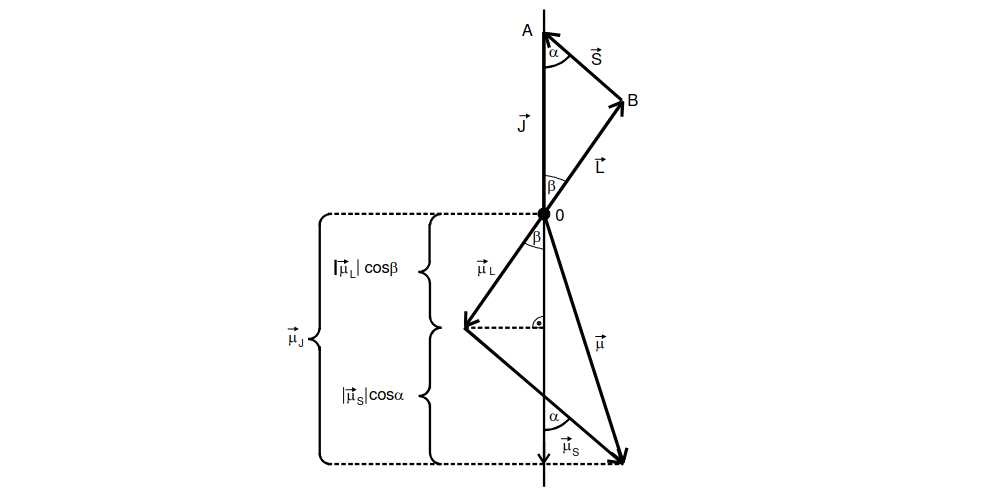
\includegraphics[width=\textwidth]{content/vec_theo.png}
    \caption{Vektorielle Darstellung der Drehimpulsvektoren einer Elektronenhülle und deren magnetischer Momente \cite{sample}.}
    \label{fig:vektoriell}
\end{figure}

Der Winkel zwischen dem externen und internen Magnetfeld $\vec{\mu_J}$ ist nach der Beziehung
\begin{equation*}
    \mu_{J_Z} = - \mu_B \cdot g_J \cdot m
\end{equation*}
gequantelt. Es sind $2J+1$ Konfigurationen einnehmbar.\\
$\mu_{J_Z}$ ist die z-Komponente des magnetischen Moments mit der ganzzahligen Orientierungsquantenzahl
$m$.\\
Über alle Konfigurationen mit den dazugehörigen Wahrscheinlichkeiten summiert
ergibt sich für die Suszeptibilität 
\begin{equation}
    \chi = \frac{\mu_0 \cdot \mu_{\text{B}}^2 \cdot g_{\text{J}}^2 \cdot N \cdot  J (J+1)}{3 \cdot k_{\text{B}} \cdot T},
    \label{eq:sus}
\end{equation} 
worin $k_B$ die Boltzmannkosntante, $N$ die Anzahl der Momente je Volumeneinheit,
und $T$ die Temperatur ist.\\
Die Gesamtdrehimpulskomponenten $L, S, \textrm{und} J$ können durch die Hundschen Regeln bestimmt werden. Diese sind:\\
1. Der Gesamtspin entsteht durch die Kombination der einzelnen Spins $\vec s_{i}$ unter Einhaltung des Pauli-Prinzips.\\
2. Der Gesamtbahndrehimpuls $\vec L =\sum \vec l_{i}$, mit den einzelnen Bahndrehimpulsen $\vec l_{i}$ setzt sich so zusammen, dass er nicht mit dem Pauli Prinzip und Regel 1 bricht. \\
3. Der Gesamtdrehimpuls $J$ bildet sich bei einer weniger als halbvollen Schale durch $\vec J=\vec L - \vec S$ und bei mehr als halbvoller Schale durch $\vec J =\vec L + \vec S$.


\subsection{Messverfahren zur Berechnung der Suszeptibilität}

Bestimmt wird die Differenz $\Delta L$ der Induktivitäten
der luftgefüllten und der mit einem paramagnetischen Stoff befüllten Spule.\\
Die Spule ist in eine Brückenschaltung verbaut, sodass aufgrund der  für hohe Frequenzen $\omega^2 L^2 >> R^2$
\begin{equation*}
    \chi (\omega \to \infty) = \frac{4 F U_\text{Br}}{Q U_\text{err}}
\end{equation*}
die Suszeptibilität durch
\begin{equation}
    \chi = \frac{2 \cdot \Delta R \cdot F}{R_3\cdot Q}
    \label{eq:alternativ}
\end{equation}
bestimmt werden kann. Hier ist $F$ der Spulenquerschnitt, $Q$ der 
Probenquerschnitt, $U_{err}$ die Erregerspannung. $\Delta R$ ist die Differenz der Potentiometereinstellungen.\\

\subsection{Selektivverstärker}

Die Güte $Q$ eines Selektivverstärkers gibt Auskunft über seine Filtereigenschaften und kann durch 
\begin{equation}
    Q = \frac{\nu_0}{\nu_+ - \nu_-}
    \label{eq:guetekuh}
\end{equation}
bestimmt werden.
Hier beschreibt $\nu_0$ die Durchlassfrequenz des Selektivverstärkers und $\nu_+$ und $\nu_-$ die Frequenzen, 
zu denen das Verhältnis $\frac{U_\text{A}}{U_\text{E}}$ den Wert $\frac{1}{\sqrt{2}}$ erreicht.\\
